\documentclass[11pt]{scrartcl}
\usepackage{titlesec}
\usepackage{graphicx}

\titleformat{\section}[block]
{\Large\bfseries\filcenter}{}{1em}{}

%opening
\title{Machine Learning - Homework 2 \\
		\vspace{+0.5cm}
		\LARGE{RoboCup 8\_Classification problem}}
\author{Gianluca Pulicati - 1708686}
\date{\vspace{-5ex}}

\begin{document}

\maketitle

\vspace{+0.01cm}
\section*{Introduction}
\noindent
\large{The second Machine Learning course's homework  has been assigned to the students of Engineering Computer Science at "Sapienza Univerità di Roma" and marks the first approach to the use of Neural Networks in a very pratical problem. \newline
The homework is based on the seminar of \textit{"Deep Ensembles \& IROS"} hold during lectures. In the seminar was discussed how Robot security is becoming important nowadays and how Deep Ensembles methodologies are useful to help ensuring this purpose. In fact, security starts from being able create a model in order to classify new instances of robot System logs as normal or abnormal thus to identify a "good" behavior from a "cyber-attacked" one. Basically with Ensemble learning is possible to train multiple models to solve the problem and then combine all the different outputs to obtain the best result.
}

\vspace{1.0cm}

\section* {Objectives}
\noindent
\large{The main object of the homework is to classify images which belong to eight different classes:}

\begin{itemize}
	\item Bouillin cup
	\item Flavored Water
	\item Latex Gloves
	\item Marshmallow bag
	\item Nectarines
	\item Pickled vegetables
	\item Plastic food containers
	\item Plastic forks
\end{itemize}

\noindent
\large{To solve this task is possible to use several different methods, although one studied during lectures is probably the most suitable: Convolutional neural network. This type of network were inspired by the connectivity pattern between neurons which resembles the organization of animal visual cortex, thus are used the most to classify images, videos, natural language processing, etc. }

\section{Dataset}
\large{The dataset given for this homework consists in eight different folders, each containing a variable number of images of the relative class. \newline
Datasets in NN are fundamental: the quantity and the quality of elements are the kernel of the NN training. \newline
The given dataset is not a huge one and it also contains some noise elements which could be useful for the model, cause it has to learn how to deal with them.} \newline

\vspace{0.5cm}

\section{Deep learning}
\noindent
\large{ \noindent The key of this homework is the use of "Deep Learning", which is an important subset of Machine Learning. \newline 
In deep learning the data is sent through different levels of neural networks, and each network hierarchically determines the specific features of the images. In other words, after processing the data, the systems finds appropriate identifiers to classify every image according to his class. A huge difference between a Machine Learning approach is that, in DL, data doesn't necessarily requires a structured/well tagged elements to use as "root" of learning process; Deep learning processes doesn't even need a human intervention meanwhile the data is crossing the layers and, at the end, the Neural network is even able to learn from his self; in fact, as a multilevel layers "algorithm", data is placed in a hierarchy of different concepts, which ultimately are able to learn from own mistakes. Meanwhile a Machine Learning algorithm would need some sort of "teaching" operations.
}

\newpage

\section{Tools and methodologies}
\noindent
\large{To accomplish this homework these are the tools used:}

\vspace{0.4cm}
\hspace{-0.1in}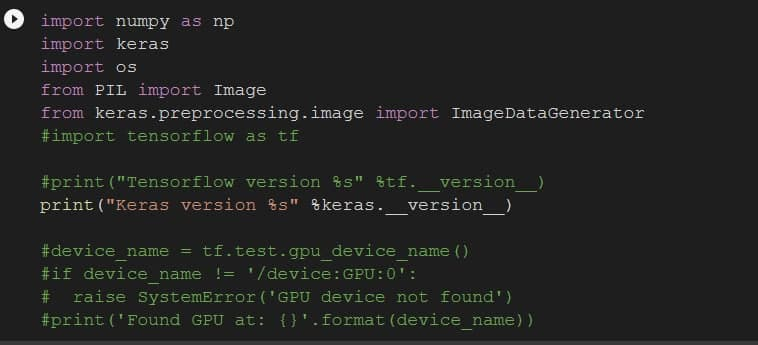
\includegraphics[width=1\textwidth]{import.png}
\vspace{0.3cm}

\noindent
\large{The Python's code above shows all the libraries used for the homework. As shown, \textit{"keras"} library is imported to solve the problem, which is a open-source library that provides an interface for artificial neural networks. \newline
Then: \newline
\textbf{PIL and os:} used to import and work with images \newline
\textbf{ImageDataGenerator:} function used to handle images in keras and run some pre-processing operations. \newline

\vspace{0.5cm}

\noindent
\textbf{\large{Note:}}\large{ The whole homework has been developed on "Google Colab", firstly to have a smooth "hardware" setup in order to test, run and debug the problem (which could be very slow on a dated computer) and also to add some layout while coding the solution. To note is the use of the "GPU" runtime provided which is an important speed-up for the training process.}

\newpage
\section{Data-set file management}


\vspace{0.4cm}
\hspace{-0.8in}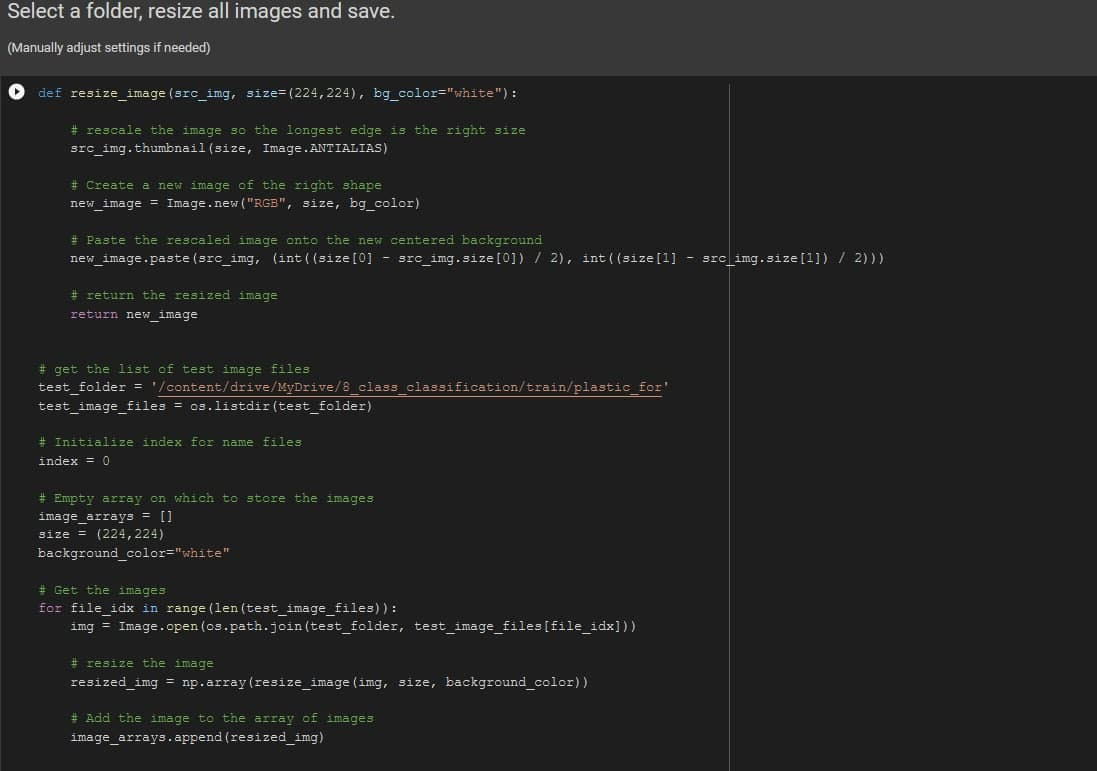
\includegraphics[width=1.3\textwidth]{datasetfile.png}
\vspace{0.3cm}

\noindent
\large{ In this piece of code is shown how dataset has been pre-processed. \newline
First of all there was the need of handling all different size of images given; basically with this function the program runs a "resize" operation on every image of the selected folder and save the new image in a new directory. To do this it create a new "white-empty background" of \textit{(224,224,3)} size to start, and then tries to adapt the original image to it. \newline
This operation is repeated for every class folder given. \newline
At the end the files are also manually splitted in two subsets: one containing the training set (70\%) and the other containing the validation set (30\%); these sets are kept fixed in order to have more comparable metrics of models.

\vspace{0.5cm}


\newpage
\section{Data generation and augmentation}

\vspace{0.4cm}
\hspace{+0.2in}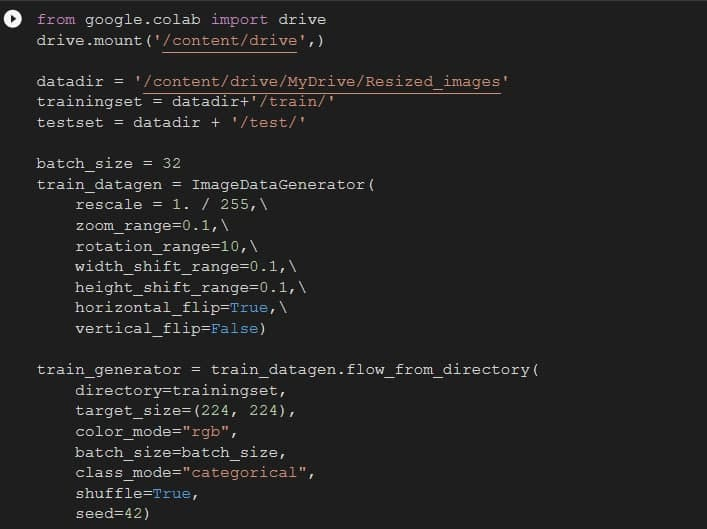
\includegraphics[width=1.0\textwidth]{datagenerator.png}
\vspace{0.3cm}

\hspace{-0.2in}\noindent
\large{ Next up there is the loading of dataset into keras.
Here batch size value is selected and then augmentation of files start: data is replaced through "flow from directory" and "image data generator" functions. \newline
Data augmentation is another fundamental step in Deep Learning; it's used to enlarge the dataset with different shape of same files. For example images are rotated, flipped and zoomed thus the Neural network will have more values to use as training elements.
This is done also for test dataset. (not shown above).
}

\newpage
\section{AlexNet model}

\begin{center}

\hspace{+0.2in}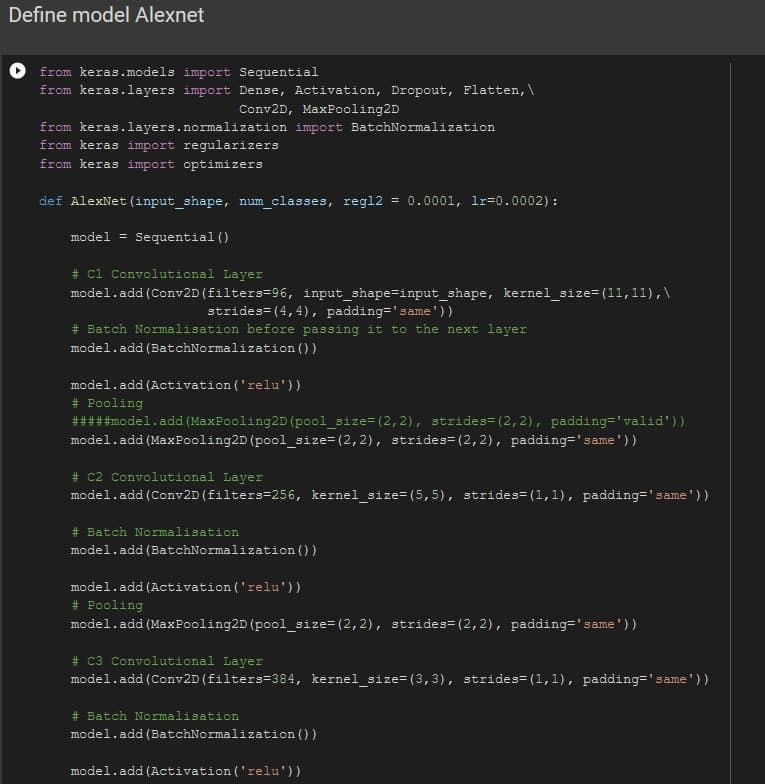
\includegraphics[width=0.7\textwidth]{Alex1.png}
\vspace{0.1cm}
\newpage
\hspace{+0.2in}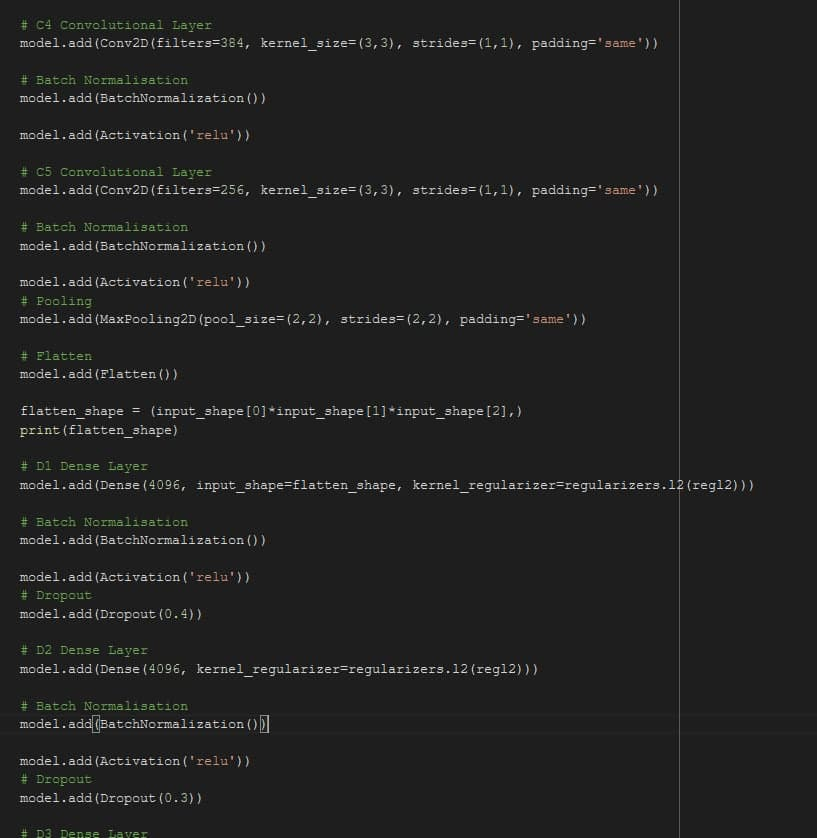
\includegraphics[width=0.7\textwidth]{Alex2.png}


\vspace{0.1cm}
\hspace{+0.2in}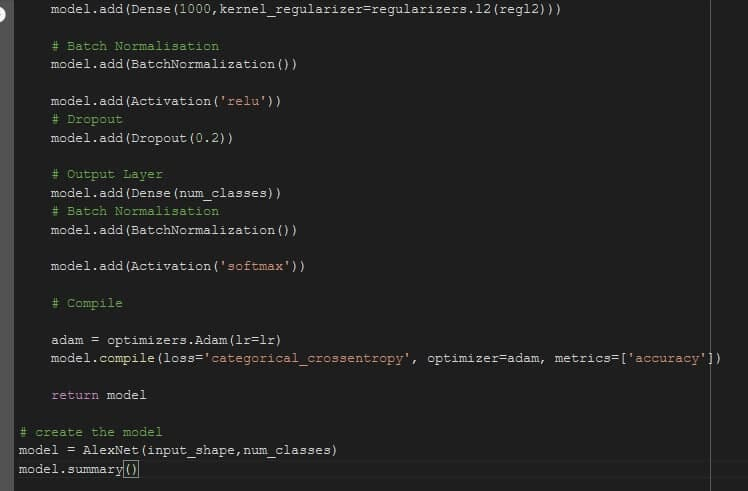
\includegraphics[width=0.7\textwidth]{Alex3.png}
\vspace{0.3cm}
\end{center}


\newpage
\section{LenNet model}

\begin{center}
	
\hspace{+0.2in}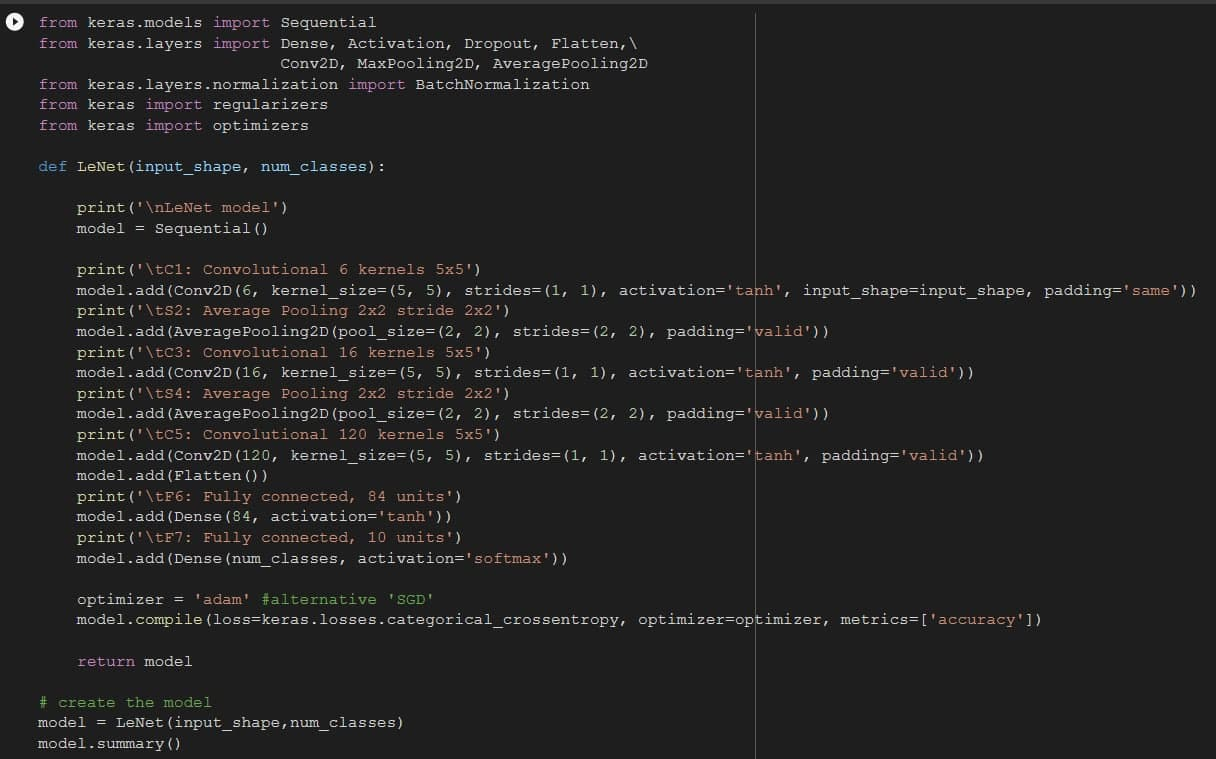
\includegraphics[width=0.8\textwidth]{lenet.png}
\vspace{0.1cm}
	
\end{center}




\newpage
\section{Conclusions}
\hspace{-0.05in}\large{

\vspace{0.5cm}

\noindent
Working with Neural network brings, in general, a set of choice that needs to be taken.
As described above, in Deep Learning one of the hardest part is to work with the data-set: building a balanced and large one is the key to have the best accuracy on the trained model. \newline
In this homework, thought, the data-set is almost fixed and pre-process' operations brings relative small changes. Since the solution develops around Neural network it's also good to not completely remove noise data; in "real life" problems every dataset has some noise, thus the model had to deal and work around it. For this reason the only pre-process' operation done in this homework was about adjusting the size of every image to a standard one, this is also to reduce the total computational time needed by the program to train the model. \newline

\vspace{0.3cm}

\noindent
The first model trained to solve the problem is "LeNet": it is composed by some Convolutional layers alternated with Pooling ones, ending with two Dense layers.
It was trained mostly with standard Batch\_size (32) value and both with a relative low epoch value (10) and high one (30). \newline
Unfortunately the accuracy level reached by the model was not very good but i expected that: LeNet was not designed to work with images of relative high resolution, in first place it was used to classify some "digits" images of about (28x28x1) size, the data-set of this homework has higher complexity which cannot be evaluated by the settings used in LeNet layers. Even trying to playing with some hyper-parameters didn't have a big impact on final metrics.

\vspace{0.3cm}

\noindent
For this reasons another model was tested: "AlexNet". At first glance was possible to check that AlexNet general settings are much more aligned to the problem we are trying to resolve. AlexNet is a CNN which uses ReLU as activation function, it takes (224x224x3) (RGB images!) as imput for first layer. Also, at the end, AlexNet has two layers fully connected with 4096 neurons each which are important cause they apply Dropout normalization. Basically with the Dropout we also let the training process "learn from noisy", when dropped out some layers output are simply ignored. This has the effect of making the layer look-like a layer with a different number of nodes to the prior layer. This simulates like a random sparse activation from a given layer and turns the system to learn from this "noise" operation! \newline
Although in this case especially playing with Dropout value had both a good and bad response. By turning the value down the model acquired slightly better accuracy point, thus brought me to the idea that the AlexNet is having some problem to learn from this noise data generated by layers, probably cause the data-self itself has a large value of "dirty" images which created some misclassification.
In general, Alexnet code provided during lectures was used for this homework, but i tried adjusting some value (especially "padding" and "strides" ones) after studying the composition of the layers of the model found on web. Also trying to edit the learning rate of loss optimizer Adam wasn't successful, slightly better results were obtained by augmenting it a little bit. (0.0002)
\newline
At the end is possible to say that even if the total accuracy (val\_accuracy) reached is not "very high", the solution provided with AlexNet at least reached a very balanced result, showing also that "plastic\_food\_container" was class creating a lot of problems and probably needed some more pre-process' operations.

\newpage
\section{AlexNet}

\begin{center}
	
	\hspace{+0.2in}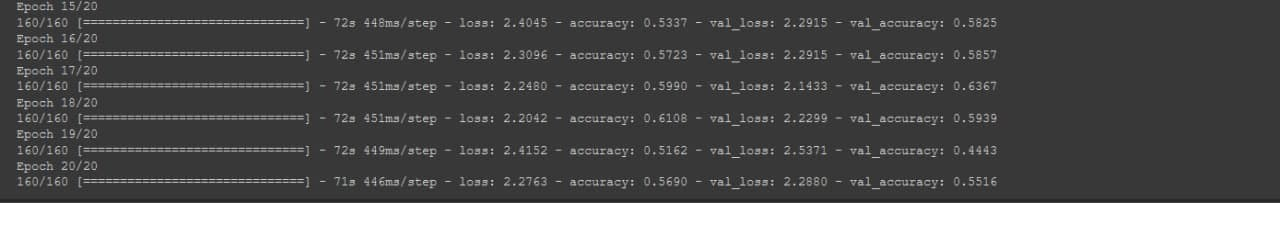
\includegraphics[width=0.7\textwidth]{dropout1.png}
	\vspace{0.1cm}
	\hspace{+0.2in}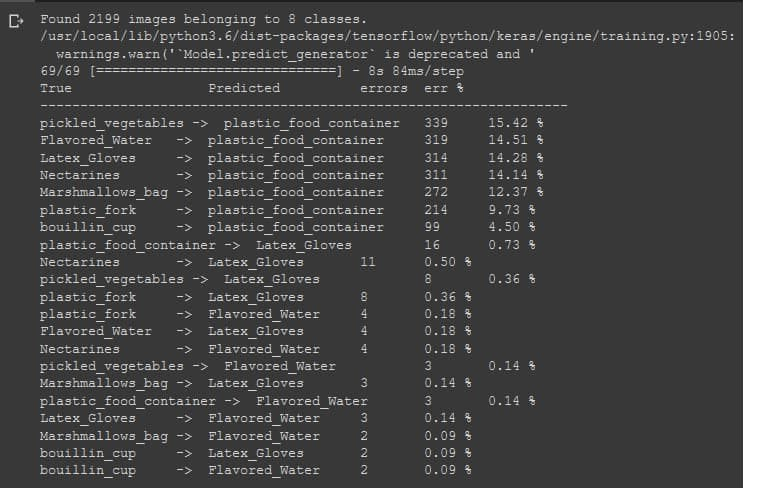
\includegraphics[width=0.7\textwidth]{Droput2.png}

\end{center}


\end{document}